% Sample file on how to use subfiles.
\documentclass[ExampleMasters.tex]{subfiles}

\begin{document}
\clearpage
{\pagestyle{empty}\cleardoublepage}%


\chapter{Software Architecture (8 Seiten)}
\label{chap:software_setup}


\section{Matlab/Simulink environment}
\label{sec:matlab}

%%\subsection{FMI toolbox}



\subsection{dSpace RTI-blockset}

The dSpace RTI-Blockset (Real-time interface) is a plug-in for MATLAB/Simulink that makes it possible to connect a simulink-model to the different inputs and outputs of the \gls{MABII} There are \gls{RTI}-blocks for CAN, Ethernet, and the analog and digital outputs of the \gls{MABII}
In this project the \gls{RTI} \gls{CAN} MultiMessage and the \gls{RTI} Ethernet (UDP) Blocksets were used.\\ 
\subsubsection{RTI \gls{CAN} MultiMessage Blockset}
The \gls{RTI} \gls{CAN} MultiMessage blocks establish an interface between the physical \gls{CAN}-Buses of the \gls{MABII} and the simulink-model running on the \gls{MABII} There are four different blocks in this blockset: A GeneralSetup-, a ControllerSetup-, a Main- and a Gateway-block. 

In the "GeneralSetup" block the paths of the model root and the destination folder for generated files are set. 

In the "ControllerSetup" block first the name of the controller has to be set. After that the physical CAN-Bus, that should be used, is set by choosing a module number and a controller number. How the module- and controller numbers have to be set for the different CAN-buses of the \gls{MABII} is shown in table \ref{tab:CAN-layout}.
\begin{table}[h]
	\centering
	\caption{CAN-layout MABII}
	\label{tab:CAN-layout}
	\begin{tabular}{c|c|c|c|c|}
		CAN   & Module number & Controller number & \gls{ZIF} -Pin CAN-High & \gls{ZIF} -Pin \gls{CAN}-Low  \\ \hline
		CAN1     &       1 & 1  & c2 & c3         \\
		CAN2   &      1 & 2  & b2 & b3    \\
		CAN3 &      2 & 1 & B2 & B3        \\
		CAN4& 2 & 2 & A2 & A3  \\
		CAN5& 3 & 1 & P2 & P3 \\
		CAN6& 3 & 2 & N2 & N3 \\
	\end{tabular} \\
\end{table}

After setting the module- and controller number the identifier format has to be set to either standard or extended format, the transceiver type must be chosen between ISO11898-2 and ISO11898-6. ISO11898-2 is used for a high-speed medium access unit and ISO11989-6 for the selective wake-up functionality of a high-speed medium access unit. If needed, a termination resistance of 120 Ohms can be set in the block as well. As a last step the Baud rate of the \gls{CAN}-bus has to be defined.


In the "Main Block" a dbc-file is connected to one of the controller blocks, that were created before. A "ControllerSetup" block \gls{CAN} only be connected to one "Main Block" at a time. When the dbc-file is loaded in the "Main Block", the different messages and signals that are specified in the dbc-file can be chosen as inputs and/or outputs of the "Main block". For signals that should be transmitted it has to be defined when they should be transmitted. There are different ways to specify this. One way is to set a cycle time in the simulink model, that determines with which frequency the signal is sent out. Another way is to use triggers that trigger the transmission every time a specific event happens. This \gls{CAN} be set in the tab "Messages" under "Triggering".

The "Gateway block" is used to gateway signals from one \gls{CAN} to another. 
\subsubsection{RTI Ethernet (UDP) Blockset}
The \gls{RTI} Ethernet (\gls{UDP}) Blockset was used for two purposes: On the one hand for the \gls{HIL} -testing (see section \ref{sec:HIL}), on the other hand for the \gls{CAN}-bus extension of the \gls{MABII} (see section \ref{sec:can_bus_extension_software}). The \gls{RTI} Ethernet (UDP) Blockset contains four different blocks: An setup-, RX-, TX-, and an interrupt-block.\\
The "Ethernet\_UDP\_SETUP" block consists of two pages. In the "Unit" page the main settings for the Ethernet are made. First the interface name has to be chosen. Then the board type has to be selected. There are two types of boards: "ETH Type 1" and "ECU Type 1 ETH". If the Ethernet cable is connected to the Ethernet port of the \gls{MABII}, "ETH Type 1" has to be chosen. The module number, which has to be set in the next step, must be set to 1 since the used \gls{MABII} only has one module.
After that, the local \gls{IP} address has to be set.\\
On the options page of the setup block up to four different sockets \gls{CAN} be enabled. For each socket a local port number, the remote ip address and the remote port number have to be set.\\
 
The "Ethernet\_UDP\_RX" block is used to receive data over Ethernet. To set up this block the board type, module number and socket number need to be set corresponding to the settings that were made in the "Ethernet \gls{UDP} Setup" block. Furthermore the maximum message size \gls{CAN} be defined. Outputs of this block are the received data, the message size and a status. The datatype of the received data is uint32. If the data wasn't transmitted as uint32 it needs to be decoded. In the demo for the Ethernet blocks a block called "DSDecode32" \gls{CAN} be found. With this block the decoding \gls{CAN} be done, by choosing the desired output data format. To get the single signals the output of that block just needs to be demuxed. If the data type of the transmitted data was already uint32 the signal \gls{CAN} be demuxed right away.

The "Ethernet\_UDP\_TX" block is used to send data over Ethernet. This \gls{CAN} be done in a similar way as for the receive block. The only difference is that in the transmit block additionally a send timeout \gls{CAN} be set. The maximum message size must match the port width of the data that is send out. It \gls{CAN} be calculated by:
\begin{equation}
data\ port\ width=(MaxMessageSize + 3) / 4
\end{equation}
The inputs to the transmit block are the data to transmit, the message size and a constant to enable the transmission. The data format of the data to transmit needs to be uint32. Similar to the receive block a so called "DSEncode" block \gls{CAN} be found in the demo for this blockset. This block encodes muxed signals of different types in a way, that they \gls{CAN} be transmitted with the transmit block. In the "DSEncode" block the data type of the different signals, that are put in the block, need to be specified.

The "Ethernet\_UDP\_INTERRUPT" \gls{CAN} be used to make the hardware interrupts available as trigger sources.
\subsection{Virtual Truck Modelling Library}
\label{sec:VTM}
The \gls{VTM} is a computational framework used within Volvo Trucks to simulate the dynamic behaviours of trucks and combinations. As a library it extends Simulink, where maneuvers, track layout and the trucks kinematic and dynamic properties are linked together and then computed. This toolbox was used as a base for the simulation of \gls{HCT} vehicles including the dolly for this project. It is possible to run simulation offline with a predefined maneuver and a given environment as well online where these parameters are fed into the calculation live or as measurings from the real-world environment. For online use all relevant parameters and states \gls{CAN} be accessed in Simulink or in case of execution on the \gls{MABII} through ControlDesk as their respective representation of the Simulink variable. 

\subsection{CAN-bus extension}
\label{sec:can_bus_extension_software}

\begin{itemize}
	\item outline data diagram structure
	\item show limitations uf \gls{UDP} (time, reliability, retrans)
	\item timestamping
	
	
\end{itemize}
\section{Steering interface}
\label{sec:steering_interface}
The steering interface block constitutes the interface between the vehicle model controller and the different \gls{CAN}s of the dolly. It is a Simulink model that runs on the \gls{MABII}
Figure \ref{fig:steering_interface} shows the steering interface block with its in- and outputs. 
\begin{figure*}[!htb]
	\centering
	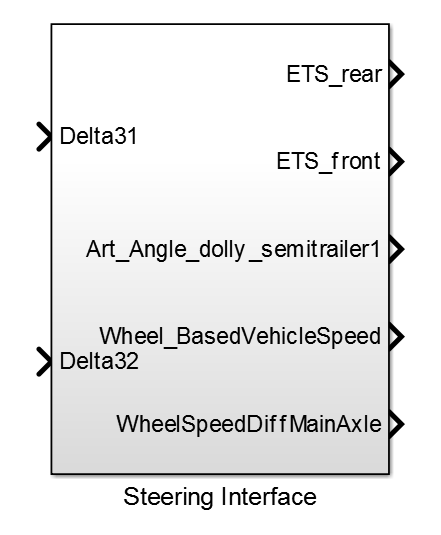
\includegraphics[width=0.5\linewidth]{figures/steering_interface}
	
	\caption{Steering interface block}
	\label{fig:steering_interface}
\end{figure*} \\
The inputs to the block are:
\begin{itemize}
	\item Delta31: Steering angle requests for front axle of the dolly 
	\item Delta32: Steering angle requests for rear axle of the dolly 
\end{itemize} 
 The outputs of the block are:
 \begin{itemize}
 	\item ETS\_rear: All signals on the \gls{ETS}-\gls{CAN} rear axle
 	\item ETS\_front: All signals on the \gls{ETS}-\gls{CAN} for front axle
 	\item Art\_Angle\_dolly\_semitrailer1: The actual articulation angle between the dolly and the first semitrailer
 	\item Wheel\_BasedVehicleSpeed: The vehicle speed signal from the dolly's \gls{EBS}
 	\item WheelSpeedDiffMainAxle: The wheel speed difference from the dolly's \gls{EBS}
 \end{itemize}
 The outputs are used to monitor the dolly's state and for the calculation of the current capabilities (see section \ref{sec:maxi_capabilities}).
 Figure \ref{fig:steering_interface_inside} shows the inside of the steering interface block. It contains \gls{RTI} \gls{CAN} MultiMessage blocks (see section \ref{RTI_CAN}).   
 
 \begin{figure*}[!htb]
 	\centering
 	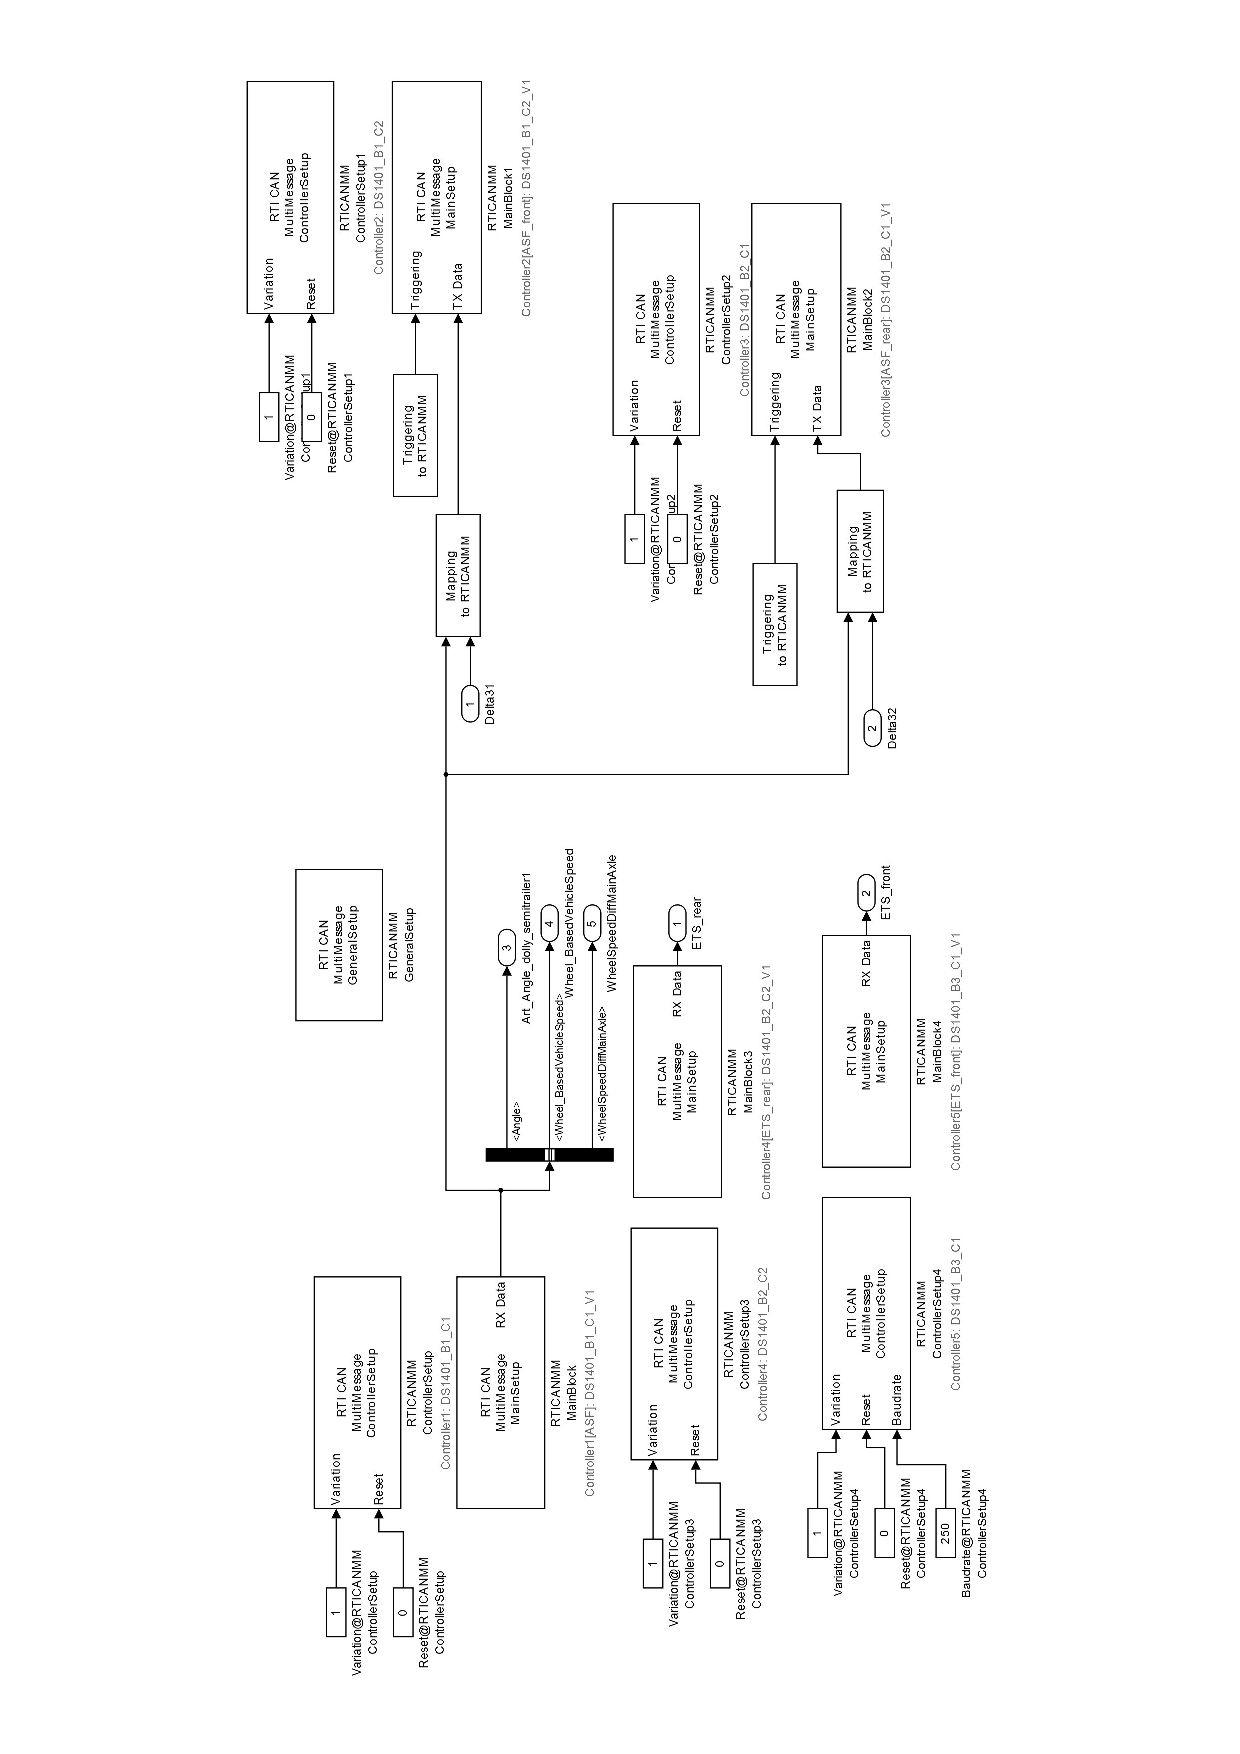
\includegraphics[width=0.95\linewidth]{figures/steering_interface_inside}
 	
 	\caption{Steering interface block \gls{CAN} layout}
 	\label{fig:steering_interface_inside_pdf}
 \end{figure*}
 
 The software CAN-layout corresponds to the hardware CAN-layout described in section \ref{sec:interface_with_dolly}. There are five different CAN-controllers. Controller1 is used to receive the signals of the ASF-Sensor and the dolly's \gls{EBS} system. These signals, except for the "Angle", "Wheel\_BasedVehicleSpeed" and the "WheelSpeedDiffMainAxle" signals are forwarded to Controller2 and Controller3. Controller2 corresponds to the \gls{ETS}-\gls{CAN} of the front axle and Controller3 to the one of the rear axle. The inputs Delta31 and Delta32 are sent to the front \gls{ETS}-\gls{CAN} (Controller2) and rear \gls{ETS}-\gls{CAN} (Controller3), respectively. For the signals "Wheel\_BasedVehicleSpeed" and  "WheelSpeedDiffMainAxle" constants with the value zero are forwarded both to Controller2 and Controller3.
 Controller4 and Controller5 also correspond to the front \gls{ETS}-\gls{CAN} and rear \gls{ETS}-\gls{CAN}, respectively. As mentioned in section \ref{sec:interface_with_dolly} this is necessary because different CAN-protocols are used. The signals received from those Controllers, together with the signals from Controller1, that weren't forwarded, are outputs of the steering interface block.
  
\section{ControlDesk monitoring environment}
\label{sec:control_desk}
The software used to monitor the Simulink model running on the \gls{MABII} and for logging of data is called dSpace ControlDesk. It also provides the possibility to control the Simulink model running on the MABII, for example by changing parameters like constants in the model during run-time. Therefore it was used for bench-testing the dolly system (see section \ref{sec:bench-testing}) to directly send steering angle request to the \gls{ETS}-\gls{CAN} via the steering interface (section \ref{sec:steering_interface}). In ControlDesk the \gls{CAN}s that the \gls{MABII} is connected to can be monitored as well. This proofed very useful for checking if all systems work correctly during early stages of development. 

\subsection{Maneuver control}
Though as mentioned in section \ref{sec:realtime_environment} the \gls{MABII} is capable of running headless and it would be possible to execute the maneuvers fully independently on start-up, it was decided to rely on manual maneuver triggering to have an extra level of safety. For controlled testing environments with clearly delimited maneuvers, the structure shown in figure \ref{fig:controlDesk_trigger} was introduced and allows to either command a steering request of zero to the dolly or patch through the calculated steering angle that is computed by the steering controller and thus starting the maneuver. 

\begin{figure*}[!htb]
	\centering
	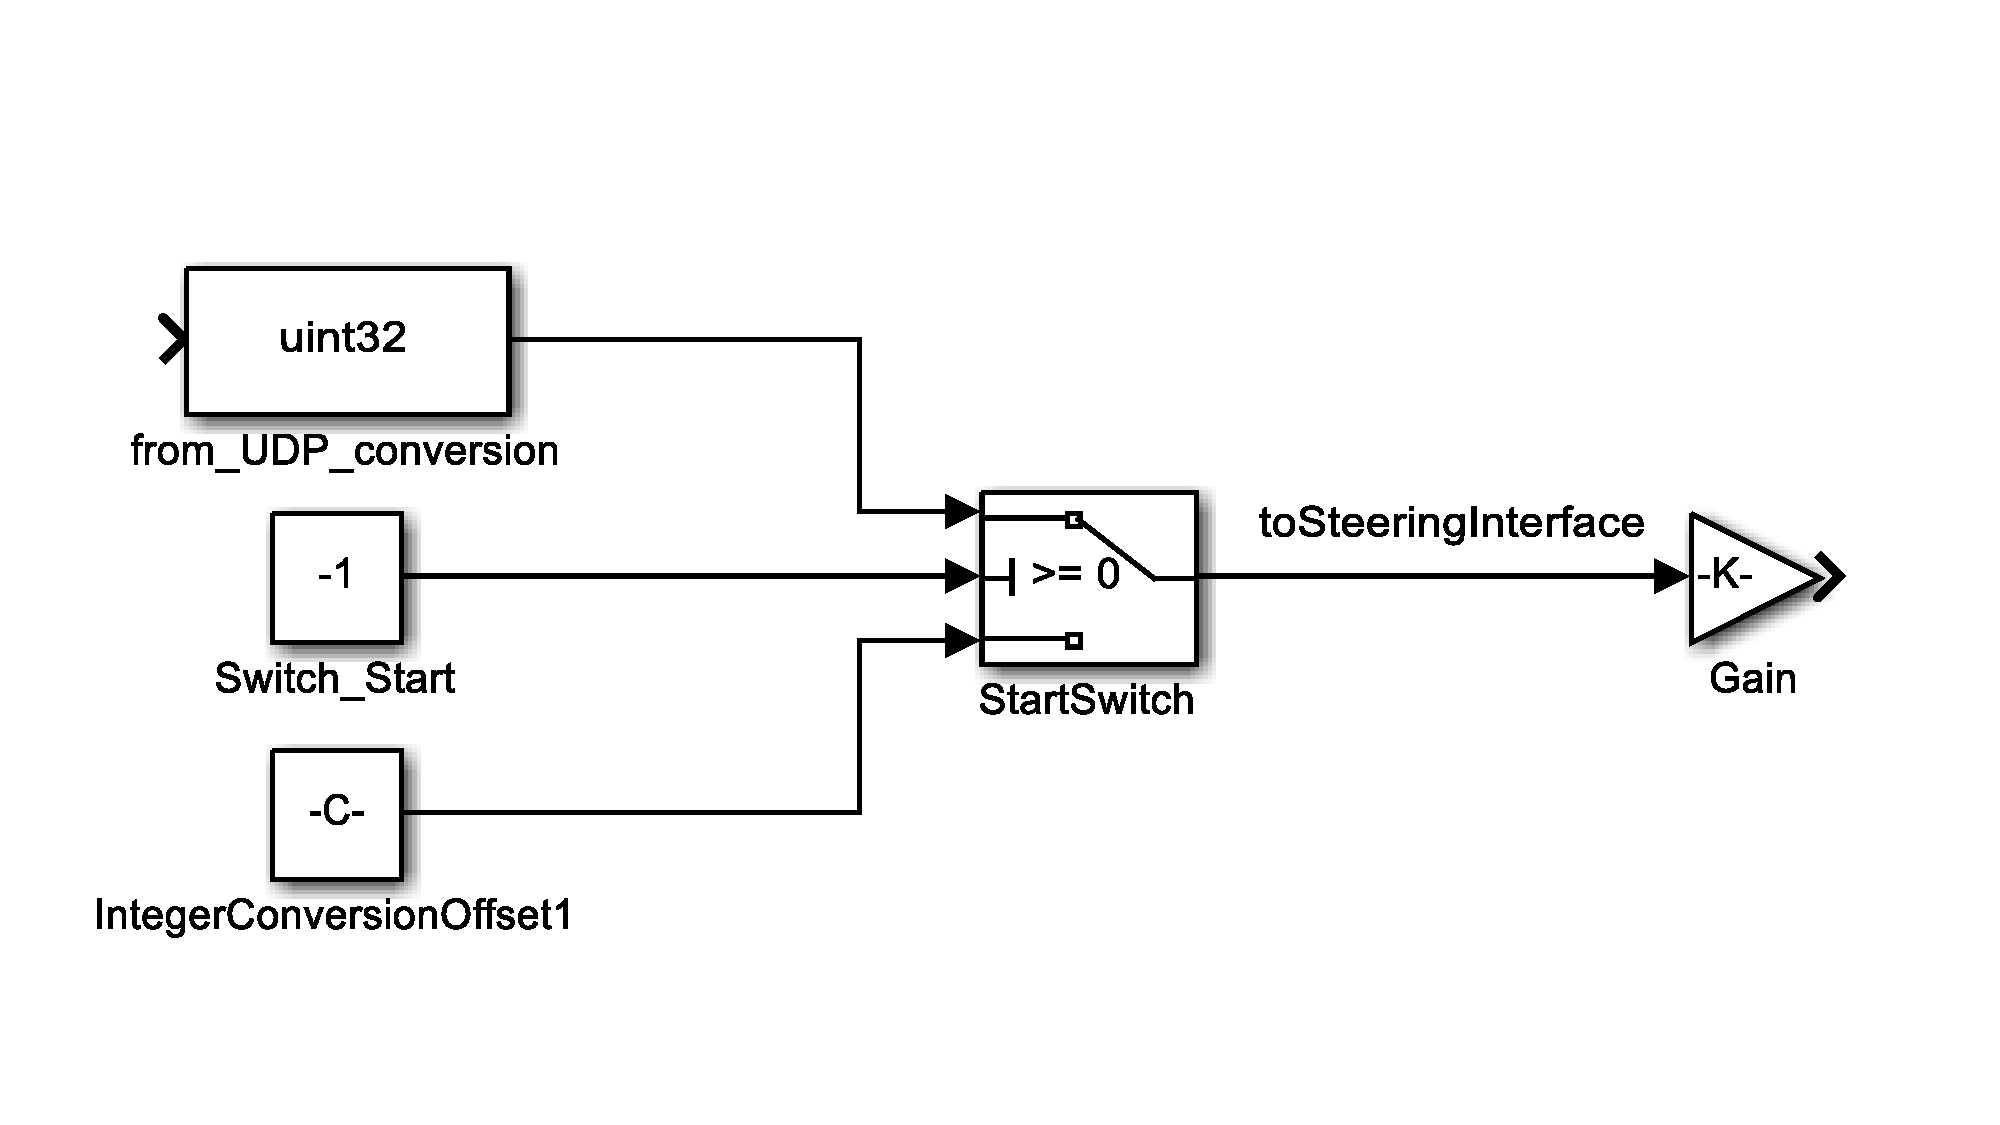
\includegraphics[width=0.6\linewidth]{figures/controlDesk_trigger}
	\caption{Trigger to start maneuver or fall back to safe-mode (e.i commanding a steering angle of zero degree on the dolly); this structure was used in \gls{HIL}-testing}
	\label{fig:controlDesk_trigger}
\end{figure*}

Sending a steering request of zero results in the dolly behaving like a passive un-steered dolly, which is also the fall-back level implemented in hardware in the legacy \gls{ETS} system. The constant block in the depicted system can be changed manually in ControlDesk to use this as a maneuver start-switch, but of course can also be accessed by the model itself. The supervisor-block can thus shutdown the steering completely on software level, preventing the triggering of the hardware-level error-mode. the hardware implementation moves the hydraulic piston of the steering system back to the middle position, if pressure is not present anymore. In doing so it enters error-mode, which needs to be reset by turning the truck's ignition off and on again. Software shutdown within the environment developed in this thesis, allows reverting back from locked mode to steering mode. 






\subsection{Monitoring and logging}
\begin{itemize}
	\item data-format
	\item frequency
	\item synchronizing over different CANs	
\end{itemize}


\section{Arduino IDE and applications}
\label{sec:arduino_applications}

The Arduino system provides an \gls{IDE}  written in Java, providing cross-platform support. It is used to develop the code as well as compiling the code and subsequently uploading it into the microcontroller via the computers serial interface. Within the IDE it is also possible to load some of the officially supported libraries directly. It conveniently is possible to monitor the computer's serial interface as well, which is the most practical way to monitor and debug code that is executed on the Arduino. 

\begin{table}[!htb]
	\label{tab:list_of_arduino_libs}
	\begin{tabular}{lll}
		\textbf{Library name} & \textbf{Purpose}                                    & \textbf{Comment} \\
		LSM303                & read magnetometer on \gls{IMU} via I2C                    &                \cite{lsm303_github}  \\
		L3G                   & read gyro \& accelerometer on \gls{IMU} via I2C           &      
		\cite{l3g_github}            \\
		UIPethernet           &     control ENC28J60 via \gls{SPI}                                                 &             \cite{uip_ethernet_github}     \\
		TinyGPSPlus           & acquire and parse GPS signal from EM-506 via serial & v0.94b\cite{tiny_gps_plus_github}     \\
		mcp\_can & implement \gls{CAN} via MCP2515 and MCP2551 via \gls{SPI}      & \cite{mcp_can_github}\\
		due\_can & implement \gls{CAN} via MCP2515 using Due's \gls{CAN}-transceiver   & \cite{due_can_github}
	\end{tabular}
	
	\caption{List of utilized libraries on the Arduino platform}
\end{table}

\end{document}
